\section{Review of Parallel Computational Models}
\label{sec:BackgroundModel}

The basic computer architecture is known as von Neummann architecture or von Neumman model. This model has the following components: a memory; an arithmetic-logic unit (ALU); a central processing unit (CPU), composed of several registers; and a control unit. New technologies and computational models began to be developed simultaneously with the evolution of the von Neumann model. 

In 1972, Michael Flynn proposed a classification of parallel computing architectures. This classification distinguishes the number of instructions and the number of data that can be computed in parallel~\citep{flynn1996parallel}. This classification is presented in the Table \ref{tab:taxFlynn}.

\begin{table}[htpb]
\begin{center}
\begin{tabular}{|r|c|c|}
\hline
& \bf Single Instruction & \bf Multiple Instruction\\\hline 
\bf Single Data & SISD & MISD \\\hline 
\bf Multiple Data & SIMD & MIMD \\\hline 
\end{tabular}
\end{center}
\caption{Classification of parallel architectures proposed by Michael Flynn (1972).} 
\label{tab:taxFlynn}
\end{table}

We can illustrate the table above as follows. A von Neumann model machine that has only one processing core fits the SISD (Single Instruction; Single Data) classification; a machine with multiple processing cores can be classified as MIMD; GPUs are classified on the SIMD architecture, where each thread takes index to perform vector computations, for this the programming model of CUDA is named SIMT (Single Instruction; Multiple Threads).

Parallel computing models have been an active research topic since the development of modern computers~\citep{Gibbons1983:QRQW,Juurlink:1998,Skillicorn:1998:MLP}; their main goal is to provide a standard way of describing and evaluating the performance of parallel applications. For the success of a parallel computing model, it is paramount to also consider the characteristics of the underlying architecture of the hardware being used.


Mathematical models are simplified abstraction of a real situation. A important area of the computer science is related with the analysis, design and development of algoritmh that are implemented in real machines. A first and general example is the RAM model (Random-Access Memory). This model is an abstraction of a classic computer with a single processor. More and not a few models were created based on the RAM model.

In computing, granularity is associated with the amount of computation in relation to communication, that is, the ratio of computation to the amount of communication. Parallelism of fine granularity means relatively small amounts of computational work are done between communication events
Low computation to communication ratio. Coarse and Bulk granularity is the opposite: data transfers are less frequent, and present large amounts of computation. Parallelism of coarse or Bulk granularity means relatively large amounts of computational work are done between communication events, high computation to communication ratio. The finer granularity have greater potential for parallelism and consequently the increase in speed, but the overhead costs of synchronization and communication are expensive in terms of latency.

The main objective of a parallel computing model is to provide a set of parameters to be considered in the implementation of a parallel algorithm. These parameters can be used to simulate the behavior of applications that will run on different parallel platforms. To facilitate the programming and simulation of these applications, models with specific properties to parallel programming problems have been created~\citep{Skillicorn:1998:MLP}. The most important parallel models in the litearature are the PRAM (Parallel Random Access Memory), LogP, BSP (Bulk Synchonous Parallel) and CGM (Coarse Grained Multicomputer). They are explained below.

\subsection{Parallel Random Access Machine Model (PRAM)}
The PRAM model was created by~\cite{Fortune:1978:PRAM}. This model is a simple extension of the RAM model. It consists of an infinite set of processors and a centralized shared memory by all processors. Figure \ref{fig:Pram} shows graphically the PRAM model

\begin{figure}[htpb]
\centering
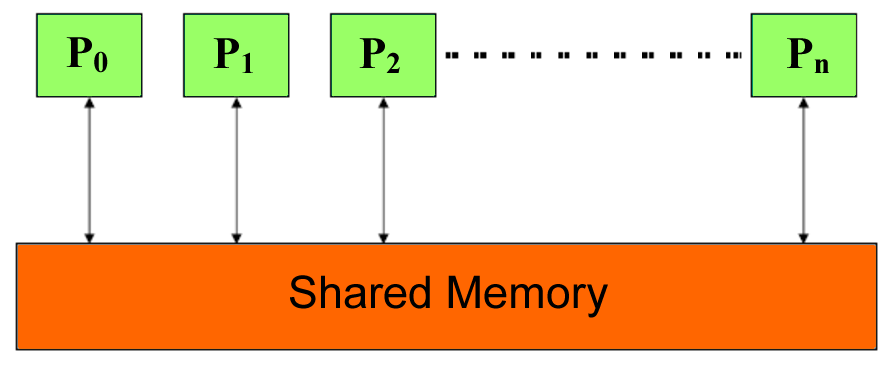
\includegraphics[scale=.6]{./images/Pram.png}
\caption{PRAM  model (\textit{Parallel Random Access Machine.})}
\label{fig:Pram}
\end{figure}

The advantage of the PRAM model is its simplicity and its similarity to the sequential model of von Neumann. The processor can only read or write a memory address in one cycle. The cost of writing is equal to the cost of reading, and is also equal to the cost of any operation performed by the processor. However, in spite of its simplicity, due to the increase in the distance between the processing and the speed of communication, this model has become more and more unrealistic.

Different submodels were created from the PRAM model. Researchers have made adaptations varying the way of access to memory, trying to avoid the maximum of conflicts in the communication. The different adaptations have arisen to propose concurrent or exclusive communications at the moment to access to shared memory~\citep{Gibbons19983:QRQW, Karp:CSD-88-408}. 

\subsection{Bulk Synchronous Parallel Model (BSP)}
The BSP model was introduced by~\cite{Valiant:1990}. The BSP model offers a simple abstraction of parallel architectures, see Figure \ref{fig:BSP}. In Figure~\ref{fig:BSP} a set of processors are running local computations in a superstep and before the synchronization, all the messages are delivered and ready to be used in the next superstep.

\begin{figure}[htpb]
\centering
% 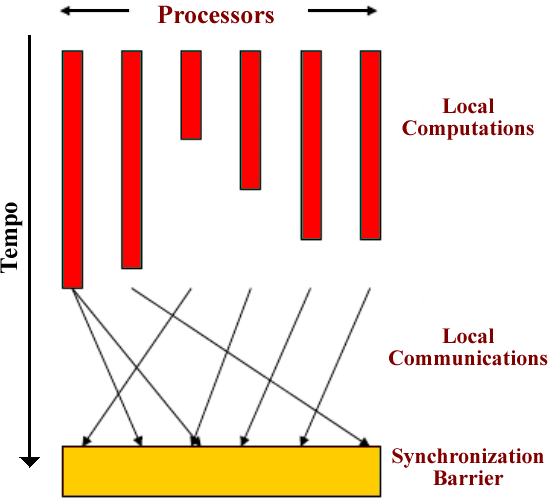
\includegraphics[scale=.7]{./images/bspmodel.eps}
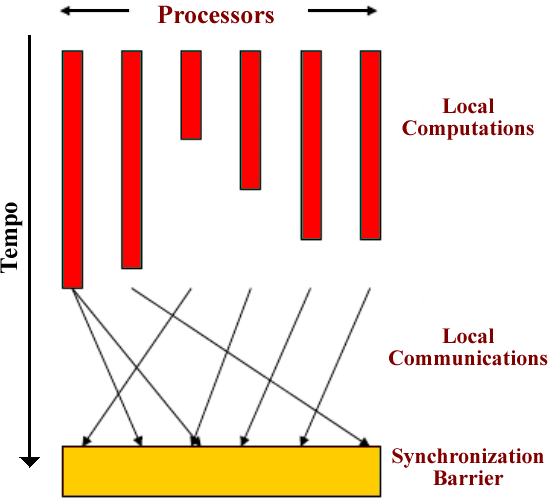
\includegraphics[scale=.7]{./images/bspmodel.png}
\caption{Superstep in a Bulk Synchronous Parallel Model.}
\label{fig:BSP}
\end{figure}

The BSP model bridges the essential characteristics of different kinds of machines as a combination of three attributes:

\begin{itemize}
\item a set of virtual processors, each associated to a local memory;
\item a router, that delivers the messages in a point-to-point manner;
\item a synchronization mechanism.
\end{itemize}

The execution of a parallel application is organized in a sequence of \emph{supersteps}, each one divided into three successive---logically disjointed---phases.
On the first phase, all processors use their local data to perform local sequential computations in parallel (i.e., there is no communication among the processors). The second phase is a communication phase, where all nodes exchange data performing personalized all-to-all communication. The last phase consists of a global synchronization barrier, that guarantees that all messages were delivered and all processors are ready to start the next superstep. 

Figure~\ref{fig:BSP} depicts the phases of a BSP application. In this figure, a processor distributes tasks to a set of processors that execute local computations and communicate in a global form, if necessary. All processors wait for the others finish their tasks in a synchronization barrier, to be able to execute the next task. Sending and receiving messages between processors is only allowed at the end of each super-step.

On the BSP model there is no restriction on sending messages, but all of them should be received before the synchronization barrier. According to the execution model, the first and second phase may occur simultaneously. A BSP algorithm consists of an arbitrary number of super-steps. The BSP model has been widely used on different applications contexts. HPC practitioners have been using the BSP model to design algorithms and software that can run on any standard architecture with guaranteed performance \cite{AlgGPU,Goldberg2004,CamargoGKG06}. Consider a BSP program that runs on $S$ supersteps. Let $g$ be the bandwidth of the network and $L$ the latency---i.e., the minimum duration of a superstep---which reflects not only the latency of the network, but also the overhead of the synchronization step. The cost to execute the $i$-th superstep is then given by:

\begin{equation}
  \label{eq:superstep-cost}
  w_i + g h_i + l
\end{equation}

where $w_i$ is the maximum amount of local computations executed, and $h_i$ is the largest number of packets sent or received by any processor during the superstep. If $W = \sum_{i=1}^{S} w_i$ is the sum of the maximum work executed on all supersteps and $H = \sum_{i=1}^{S} h_i$ the sum of the maximum number of messages exchanged in each superstep, then the total execution time of the parallel application is given by:
\begin{equation}
  \label{ec:BSP}
  T = W + g H + L S
\end{equation}

A BSP algorithm, consequently, can be completely modeled by the parameters $(w, h, g, l)$. Using these parameters, the approximate execution time of a BSP algorithm can be characterized. One of the great advantages of the BSP model is that it facilitates to develop parallel programs on different systems and architectures, serving as a bridge between the programmer who develop parallel applications in massively parallel architectures.

\subsubsection{Multi-BSP model}
The Multi-BSP model is an adaptation of the BSP model, the BSP model is commonly used in a distributed memory parallel environment, and multi-BSP is a BSP extension for multi-core processors. ~\cite{Valiant:2011} created the Multi-BSP model which is used in a parallel shared memory environment. Computational models, such as multi-BSP, allow abstraction of the complexity of the problem in a simplification that is not significantly away from the reality of current computational  architectures.  

Multi-BSP is a multi-level model that has explicit parameters at each level: number of processors $p$, memory/cache sizes $m$, communication latency costs $g$ and synchronization costs $L$. The multi-BSP model of an architecture with depth $d$ will be determined by $4d$ numeric parameters, $(p1, g1, L1, m1), (p2, g2, L2, m2), ( P3, g3, L3, m3), ..., (pd, gd, Ld, md)$. At each level the four parameters quantify, respectively, the number of subcomponents, processors, communication bandwidth, synchronization cost, and memory/cache size~\citep{BSPMeasures}.

Multi-BSP and BSP are important models that allow bridging the analysis, design and development of parallel algorithms, but they are not useful to design algorithms that are executed in massively parallel architectures. New models of performance prediction of applications that run on GPUs have arisen from adaptations of the models in this literature review.

\subsection{Coarse Grained Multicomputer Model (CGM)}
\cite{Dehne:2002} studied the problem of designing scalable parallel geometric algorithms for coarse grained cases. They called this model as Coarse Grained Multicomputer model (CGM), which is very efficient for a large set of problems of the ratio $\frac{n}{p}$, with $n$ the size of the problem and $p$ the number of processors. In other words, the CGM model is very good for addressing problems where the problem of size $n$ can be divided between an determined number of processors $p$. A CGM algorithm is a special case of a BSP algorithm where all communication operations of a super-step are done in $h$ relations. A fundamental difference between the BSP model and CGM is that the first captures real machine parameters while the CGM is an abstraction that allows to develop efficient algorithms in parallel machines.

An algorithm on a CGM machine can be modeled using only two parameters, $N$ and $p$. This algorithm consists of an alternating sequence of computing and communication rounds also separated by a synchronization barrier. A computational/communication round of the CGM model corresponds to a super-step of the BSP model with communication cost $g(N/p)$. A good performance of algorithms with the CGM model is achieved by minimizing the number of super-steps, the total time of local computations and the total size of the messages.

\subsection{LogP Model}
Synchronization of a large group of processes or threads is expensive in terms of latency, especially on architectures with classification MIMD. For these cases, parallel computing models without synchronization were created. The most popular of these models is the logP model.

LogP model was proposed by \citet{Culler:1993:LogP} and received its name exactly for the variables of the model. Culler et. al. perceived that the PRAM model was not realistic due to the lack of parameters to represent communication costs in parallel applications, especially for distributed applications. The parameters used to describe a parallel system according to LogP model are:

\begin{itemize}
\item[L:] \textit{Latency} - caused by communicating a message from a source to a destiny processor.
\item[o:] \textit{Overhead} - time during which a processor is busy sending or receiving a message, during that time it can not do
computations.
\item[g:] \textit{Gap} - minimum time between consecutive message transmissions or between receiving consecutive messages; the reciprocal of $g$ corresponds to the bandwidth of the system.
\item[P:] \textit{Processors}.
\end{itemize}

